% Author: Izaak Neutelings (June, 2018)
\documentclass[border=3pt,tikz]{standalone}
\usepackage{ifthen}
\usepackage{siunitx}
\usepackage{tikz}
\usetikzlibrary{hobby} % for ..
\usetikzlibrary{arrows.meta} % to control arrow size
\tikzset{>={Latex[length=4,width=4]}} % for LaTeX arrow head
\usetikzlibrary{calc,intersections,decorations.markings}
\usepackage{siunitx}
\usepackage{xcolor} % for colored text

\colorlet{mylightblue}{blue!20}
\colorlet{myblue}{blue!50!black}
\colorlet{mydarkblue}{blue!30!black}
\colorlet{mylightred}{red!10}
\colorlet{myred}{red!50!black}
\colorlet{mydarkred}{red!60!black}
\colorlet{mydarkgreen}{green!30!black}

%\tikzstyle{midarr}=[decoration={markings,mark=at position 0.5 with {\arrow{stealth}}},postaction={decorate}]
\tikzset{
  midarr/.style={decoration={markings,mark=at position #1 with {\arrow{stealth}}},postaction={decorate}},
  midarr/.default=0.5
}
\def\tick#1#2{\draw[thick] (#1) ++ (#2:0.03*\ymax) --++ (#2-180:0.06*\ymax)}

\begin{document}


% PHASE DIAGRAM
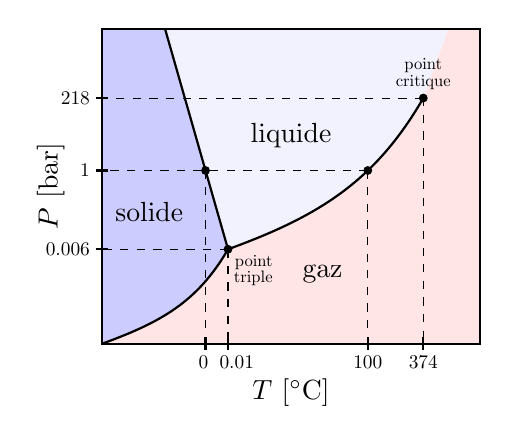
\begin{tikzpicture}[scale=0.4]
	\message{Phase diagrams^^J}

	\def\xtick#1#2{\draw[thick] (#1)++(0,.2) --++ (0,-.4) node[below=-.5pt,scale=0.7] {#2};}
	\def\ytick#1#2{\draw[thick] (#1)++(.2,0) --++ (-.4,0) node[left=-.5pt,scale=0.7] {#2};}

	% COORDINATES
	\coordinate (O) at (0,0);
	\coordinate (N1) at (2,10);
	\coordinate (N2) at (11,10);
	\coordinate (NE) at (12,10);
	\coordinate (NW) at (0,10);
	\coordinate (SE) at (12,0);
	\coordinate (W) at (0,5);
	\coordinate (S) at (6,0);
	\coordinate (C) at (10.2,7.8); % critical
	\coordinate (T) at (4,3); % triple

	% PATHS
	\def\SL{(T) -- (N1)}
	\def\SG{(O) to[out=20,in=-120] (T)}
	\def\LG{(T) to[out=20,in=-120] (C)}
	\def\atm{(0,5.5) -- (12,5.5)}
	\path[name path=SL] \SL;
	\path[name path=LG] \LG;
	\path[name path=atm] \atm;

	% REGIONS
	\fill[mylightblue] \SG -- (N1) -- (NW) -- cycle;
	\fill[blue!5] \LG -- (N2) -- (N1) -- cycle;
	\fill[mylightred] \LG -- (N2) -- (NE) -- (SE) -- \SG -- cycle;
	\node at (1.5,4.2) {solide};
	\node at (7,2.2) {gaz};
	\node at (6,6.6) {liquide};

	%% MIXED
	%\shade[top color=mylightblue,bottom color=mylightred,shading angle=70]
	%  (10.4,7.7) -- (11.2,10) -- (10.8,10) -- (10.0,7.7) -- cycle;

	% POINTS
	\fill[black,name intersections={of=SL and atm,by=M}] (M) circle (4pt);
	\fill[black,name intersections={of=LG and atm,by=B}] (B) circle (4pt);
	\fill (T) circle (4pt) node[below right,scale=0.6,align=right]
		{point\\[-2pt]triple};
	\fill (C) circle (4pt) node[above=1pt,scale=0.6,align=center]
		{point\\[-2pt]critique};

	% LINES
	\draw[thick] \SG;
	\draw[thick] \LG;
	\draw[thick] \SL;
	\draw[dashed] (M) -- ($(M |- 0,0)$) coordinate (Mx);
	\draw[dashed] (T) -- ($(T |- 0,0)$) coordinate (Tx);
	\draw[dashed] (T) -- ($(T -| 0,0)$) coordinate (Ty);
	\draw[dashed] (B) -- ($(B |- 0,0)$) coordinate (Bx);
	\draw[dashed] (B) -- ($(B -| 0,0)$) coordinate (By);
	\draw[dashed] (C) -- ($(C |- 0,0)$) coordinate (Cx);
	\draw[dashed] (C) -- ($(C -| 0,0)$) coordinate (Cy);

	% AXES
	\draw[thick] (O) rectangle (NE);
	\node[left=10pt,above,rotate=90] at (W) {$P$ [bar]};
	\node[below=9pt] at (S) {$T$ [\si{\degreeCelsius}]};
	\xtick{Mx}{\hspace{-2pt}0}
	\xtick{Tx}{\hspace{9pt}0.01}
	\ytick{Ty}{0.006}
	\xtick{Bx}{100}
	\ytick{By}{1}
	\xtick{Cx}{374}
	\ytick{Cy}{218}

\end{tikzpicture}


\end{document}
